% in this file I leave the figure captions outside\ caption{} because I want them
% to be formatted in the same way as the general text (double spaced and linenumbered)
\captionsetup[figure]{labelfont={sc},labelformat={default},labelsep=period,name={Figure}}

%%%%%%%%%%%%%%%%%%%%%%%%%%%%%%%%%%%%%%%%%%%%%%%%%%%%%%%%%%%%%%%%%%
%%%%%%%%%%%%%%%%%%%%%%%%    FIGURE 1    %%%%%%%%%%%%%%%%%%%%%%%%%%
%%%%%%%%%%%%%%%%%%%%%%%%%%%%%%%%%%%%%%%%%%%%%%%%%%%%%%%%%%%%%%%%%%
\begin{figure}[!h]
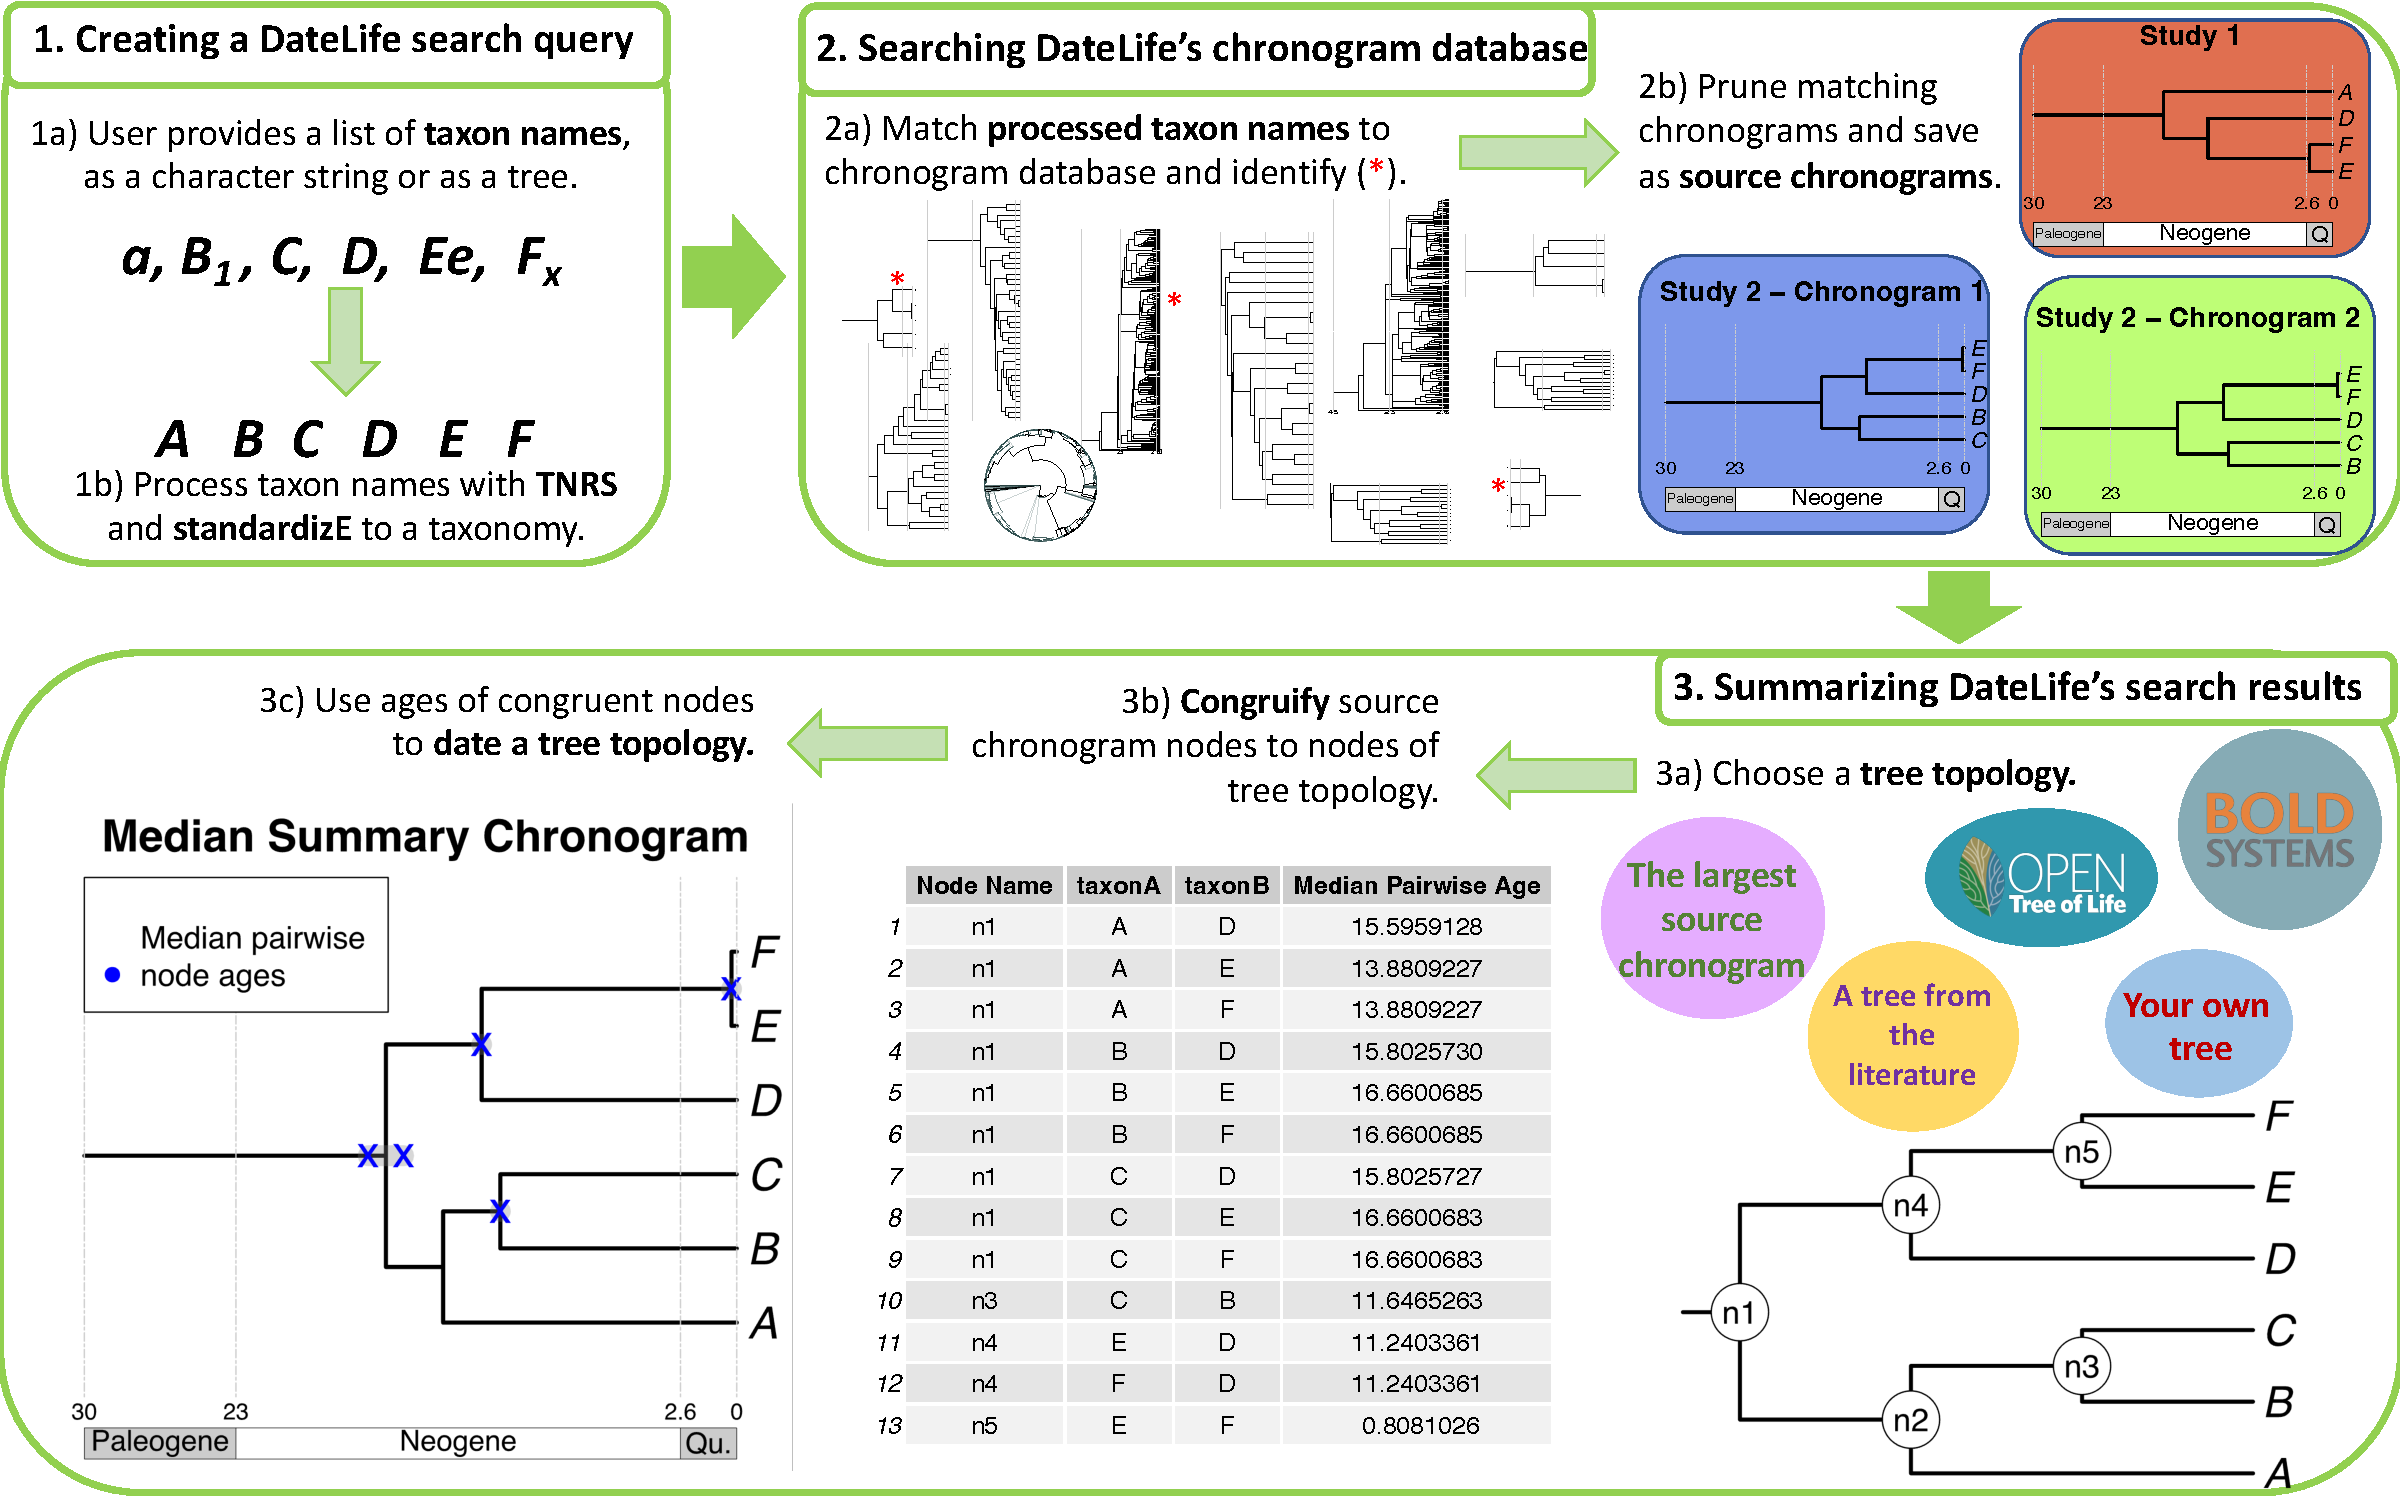
\includegraphics{../figures/figure1/figure1-new.pdf}
\caption{Stylized DateLife workflow. This shows the general worflows and analyses that can be performed with \texttt{datelife}, via the R package or through the website  at \url{http://www.datelife.org/}. Details on the functions involved on each workflow are shown in \texttt{datelife}'s R package vignette.
}
\label{fig:workflow}
\end{figure}


%%%%%%%%%%%%%%%%%%%%%%%%%%%%%%%%%%%%%%%%%%%%%%%%%%%%%%%%%%%%%%%%%%
%%%%%%%%%%%%%%%%%%%%%%%%    FIGURE runtime    %%%%%%%%%%%%%%%%%%%%
%%%%%%%%%%%%%%%%%%%%%%%%%%%%%%%%%%%%%%%%%%%%%%%%%%%%%%%%%%%%%%%%%%
\begin{figure}[!h]
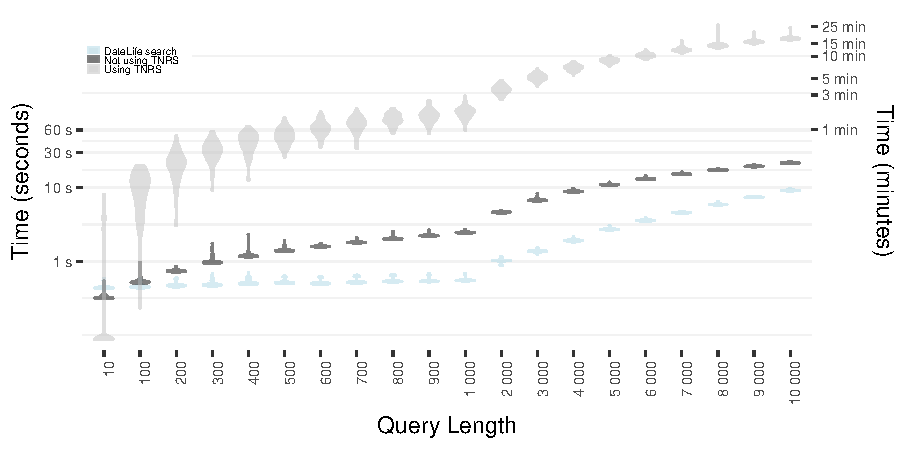
\includegraphics[width=1\linewidth]{../figures/fig_runtime_main.pdf}
\caption{Computation time of query processing and search across \texttt{datelife}'s chronogram database relative to number of input taxon names. We sampled N names from the class Aves for each cohort 100 times and then performed a search with query processing not using the Taxon Names Resoultion Service (TNRS; dark gray), and using TNRS (light gray). We also performed a search using the already processed query for comparison (light blue).}
\label{fig:runtime_main}
\end{figure}


%%%%%%%%%%%%%%%%%%%%%%%%%%%%%%%%%%%%%%%%%%%%%%%%%%%%%%%%%%%%%%%%%%
%%%%%%%%%%%%%%%%%%%%%%%%    FIGURE 2    %%%%%%%%%%%%%%%%%%%%%%%%%%
%%%%%%%%%%%%%%%%%%%%%%%%%%%%%%%%%%%%%%%%%%%%%%%%%%%%%%%%%%%%%%%%%%
\begin{figure}[!h]
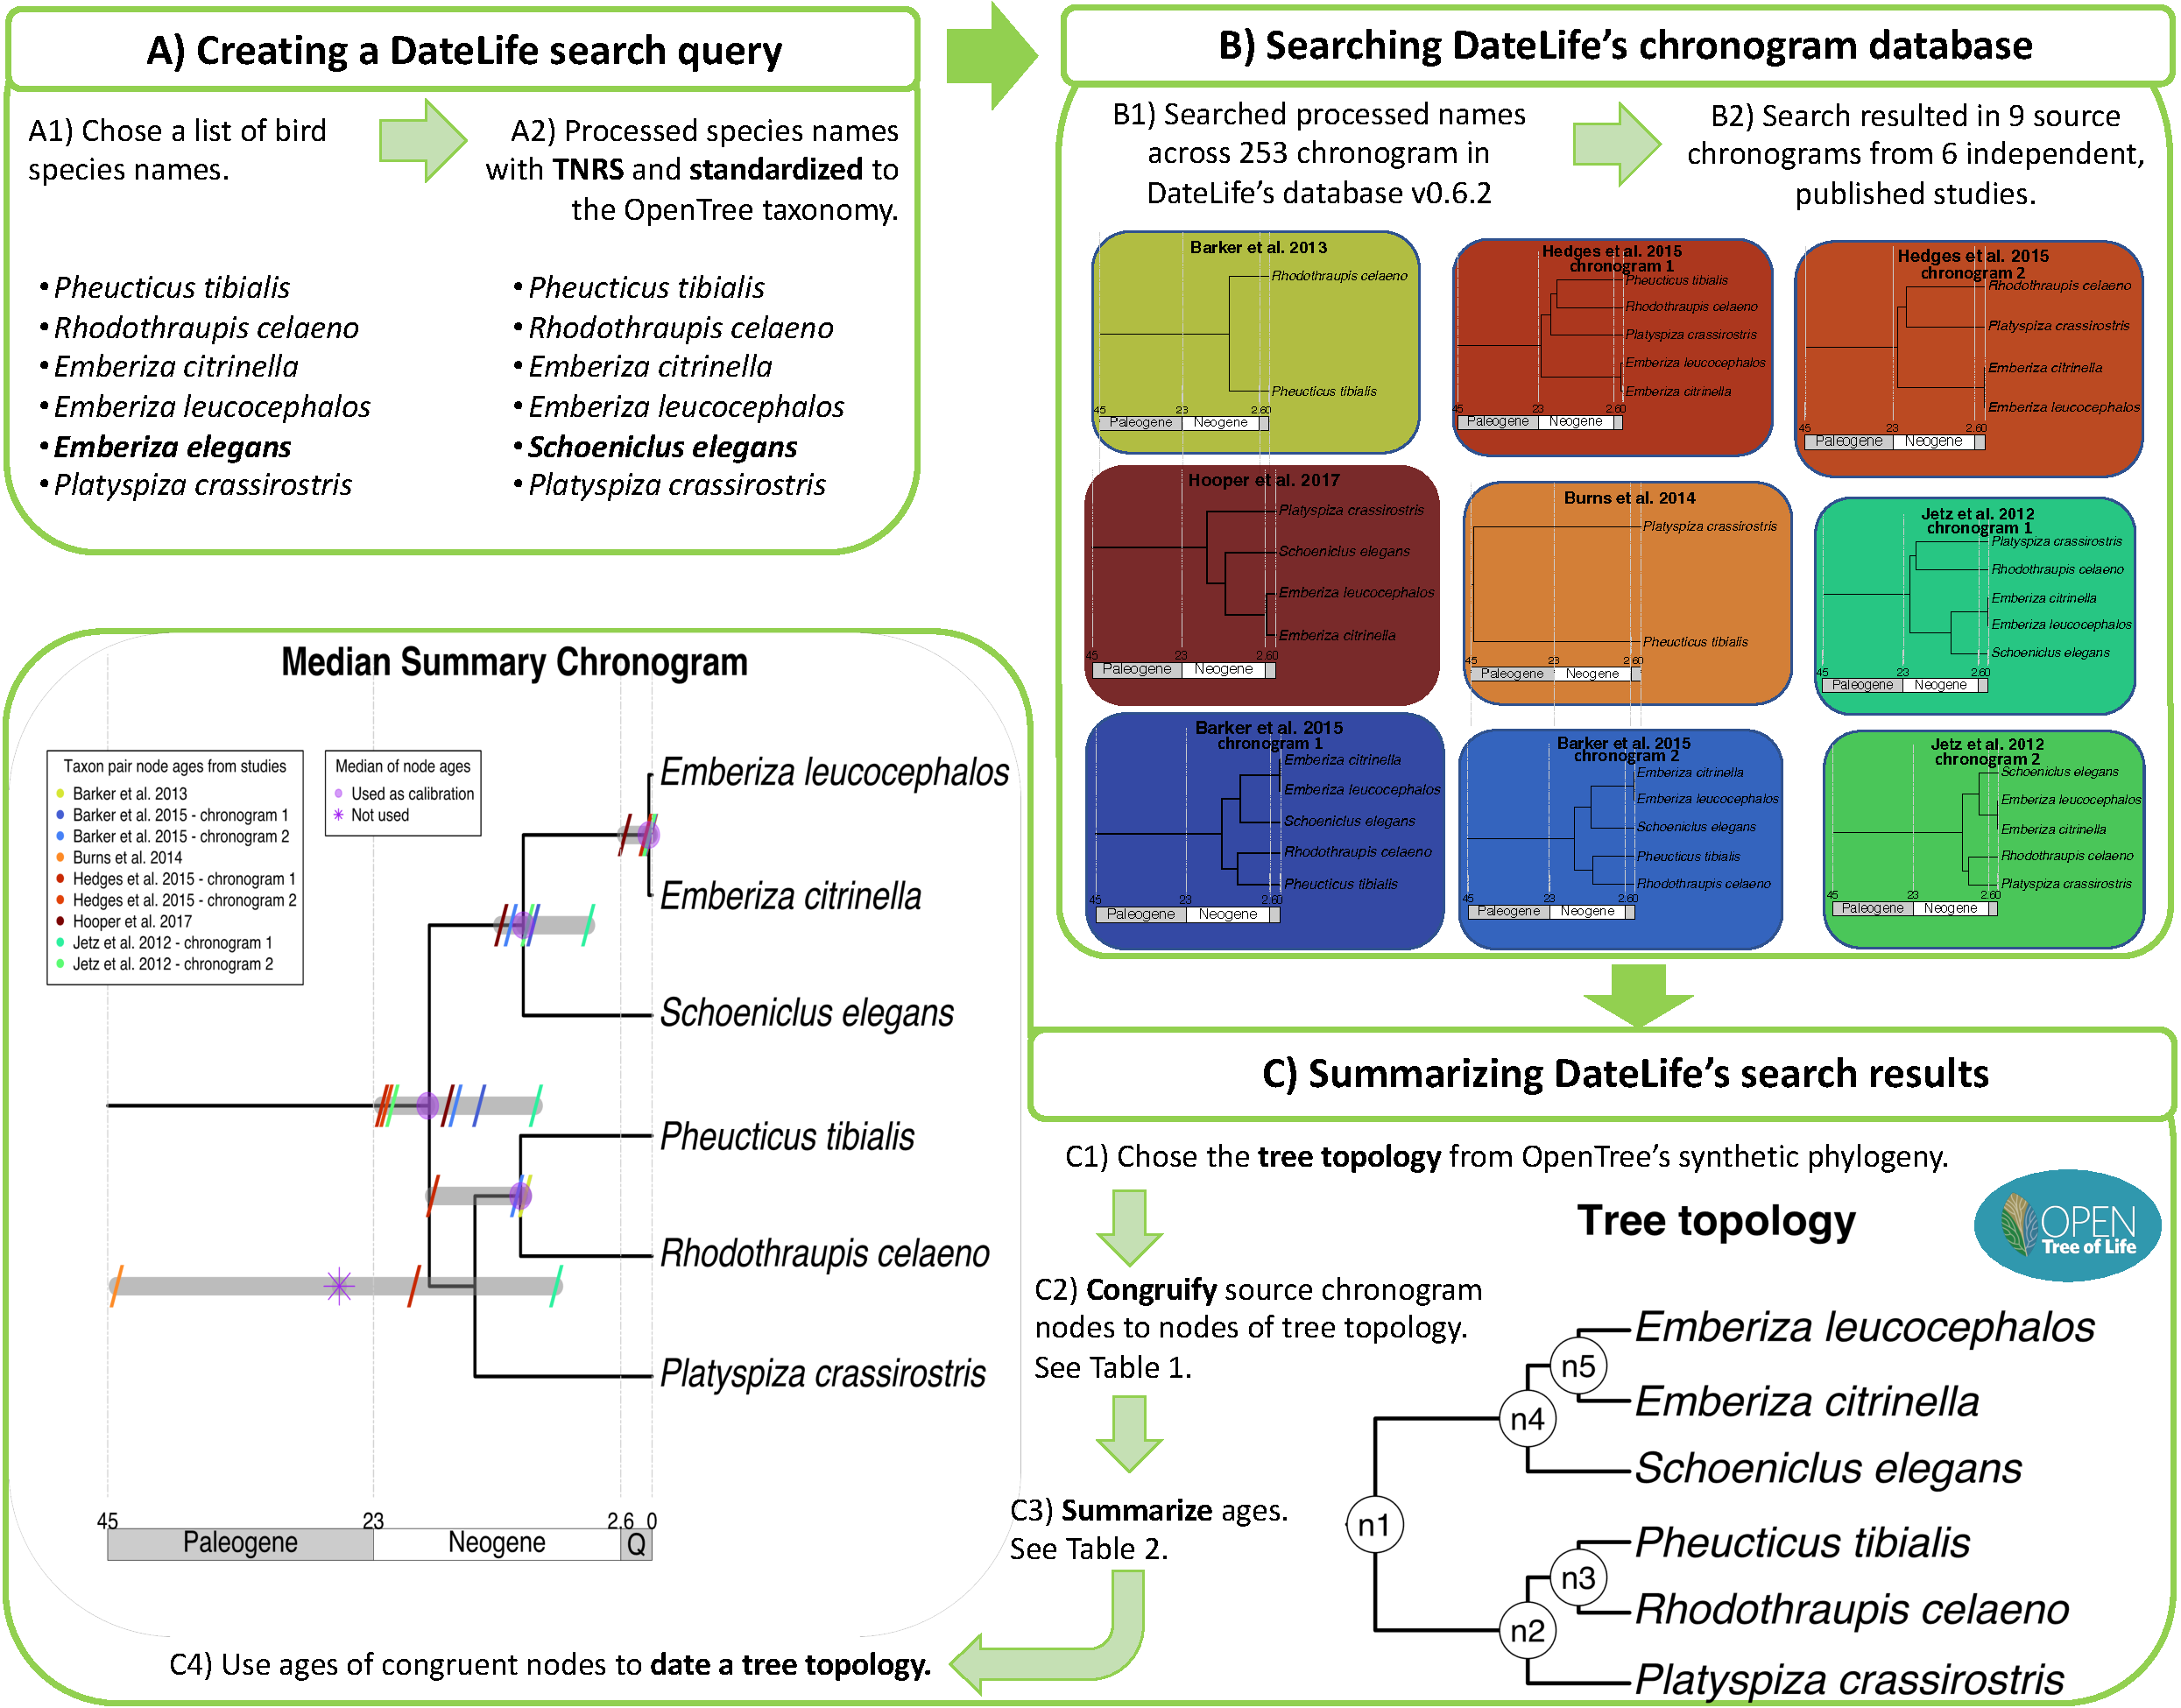
\includegraphics[width=1\linewidth]{../figures/figure2/figure2.pdf}
\caption{DateLife analysis results for a small sample of A) 6 bird species within the Passeriformes. B) Processed species names were found across 9 chronograms within 6 independent studies (Barker et al. (\protect\hyperlink{ref-barker2012going}{2012}), Barker et al. (\protect\hyperlink{ref-barker2015new}{2015}), Burns et al. (\protect\hyperlink{ref-burns2014phylogenetics}{2014}), Hedges et al. (\protect\hyperlink{ref-Hedges2015}{2015}), Hooper and Price (\protect\hyperlink{ref-hooper2017chromosomal}{2017}), Jetz et al. (\protect\hyperlink{ref-Jetz2012}{2012}).) C) This revealed 28 source age data points for the queried species names. Summarized age data is used as secondary calibrations to date a tree topology obtained from OpenTree's synthetic tree, resulting in a summary chronogram of source ages.}
\label{fig:figure2}
\end{figure}


%%%%%%%%%%%%%%%%%%%%%%%%%%%%%%%%%%%%%%%%%%%%%%%%%%%%%%%%%%%%%%%%%%%
%%%%%%%%%%%%%%%%%%%%%%%%%    FIGURE 2-1  %%%%%%%%%%%%%%%%%%%%%%%%%%
%%%%%%%%%%%%%%%%%%%%%%%%%%%%%%%%%%%%%%%%%%%%%%%%%%%%%%%%%%%%%%%%%%%
%\begin{figure}[!h]
%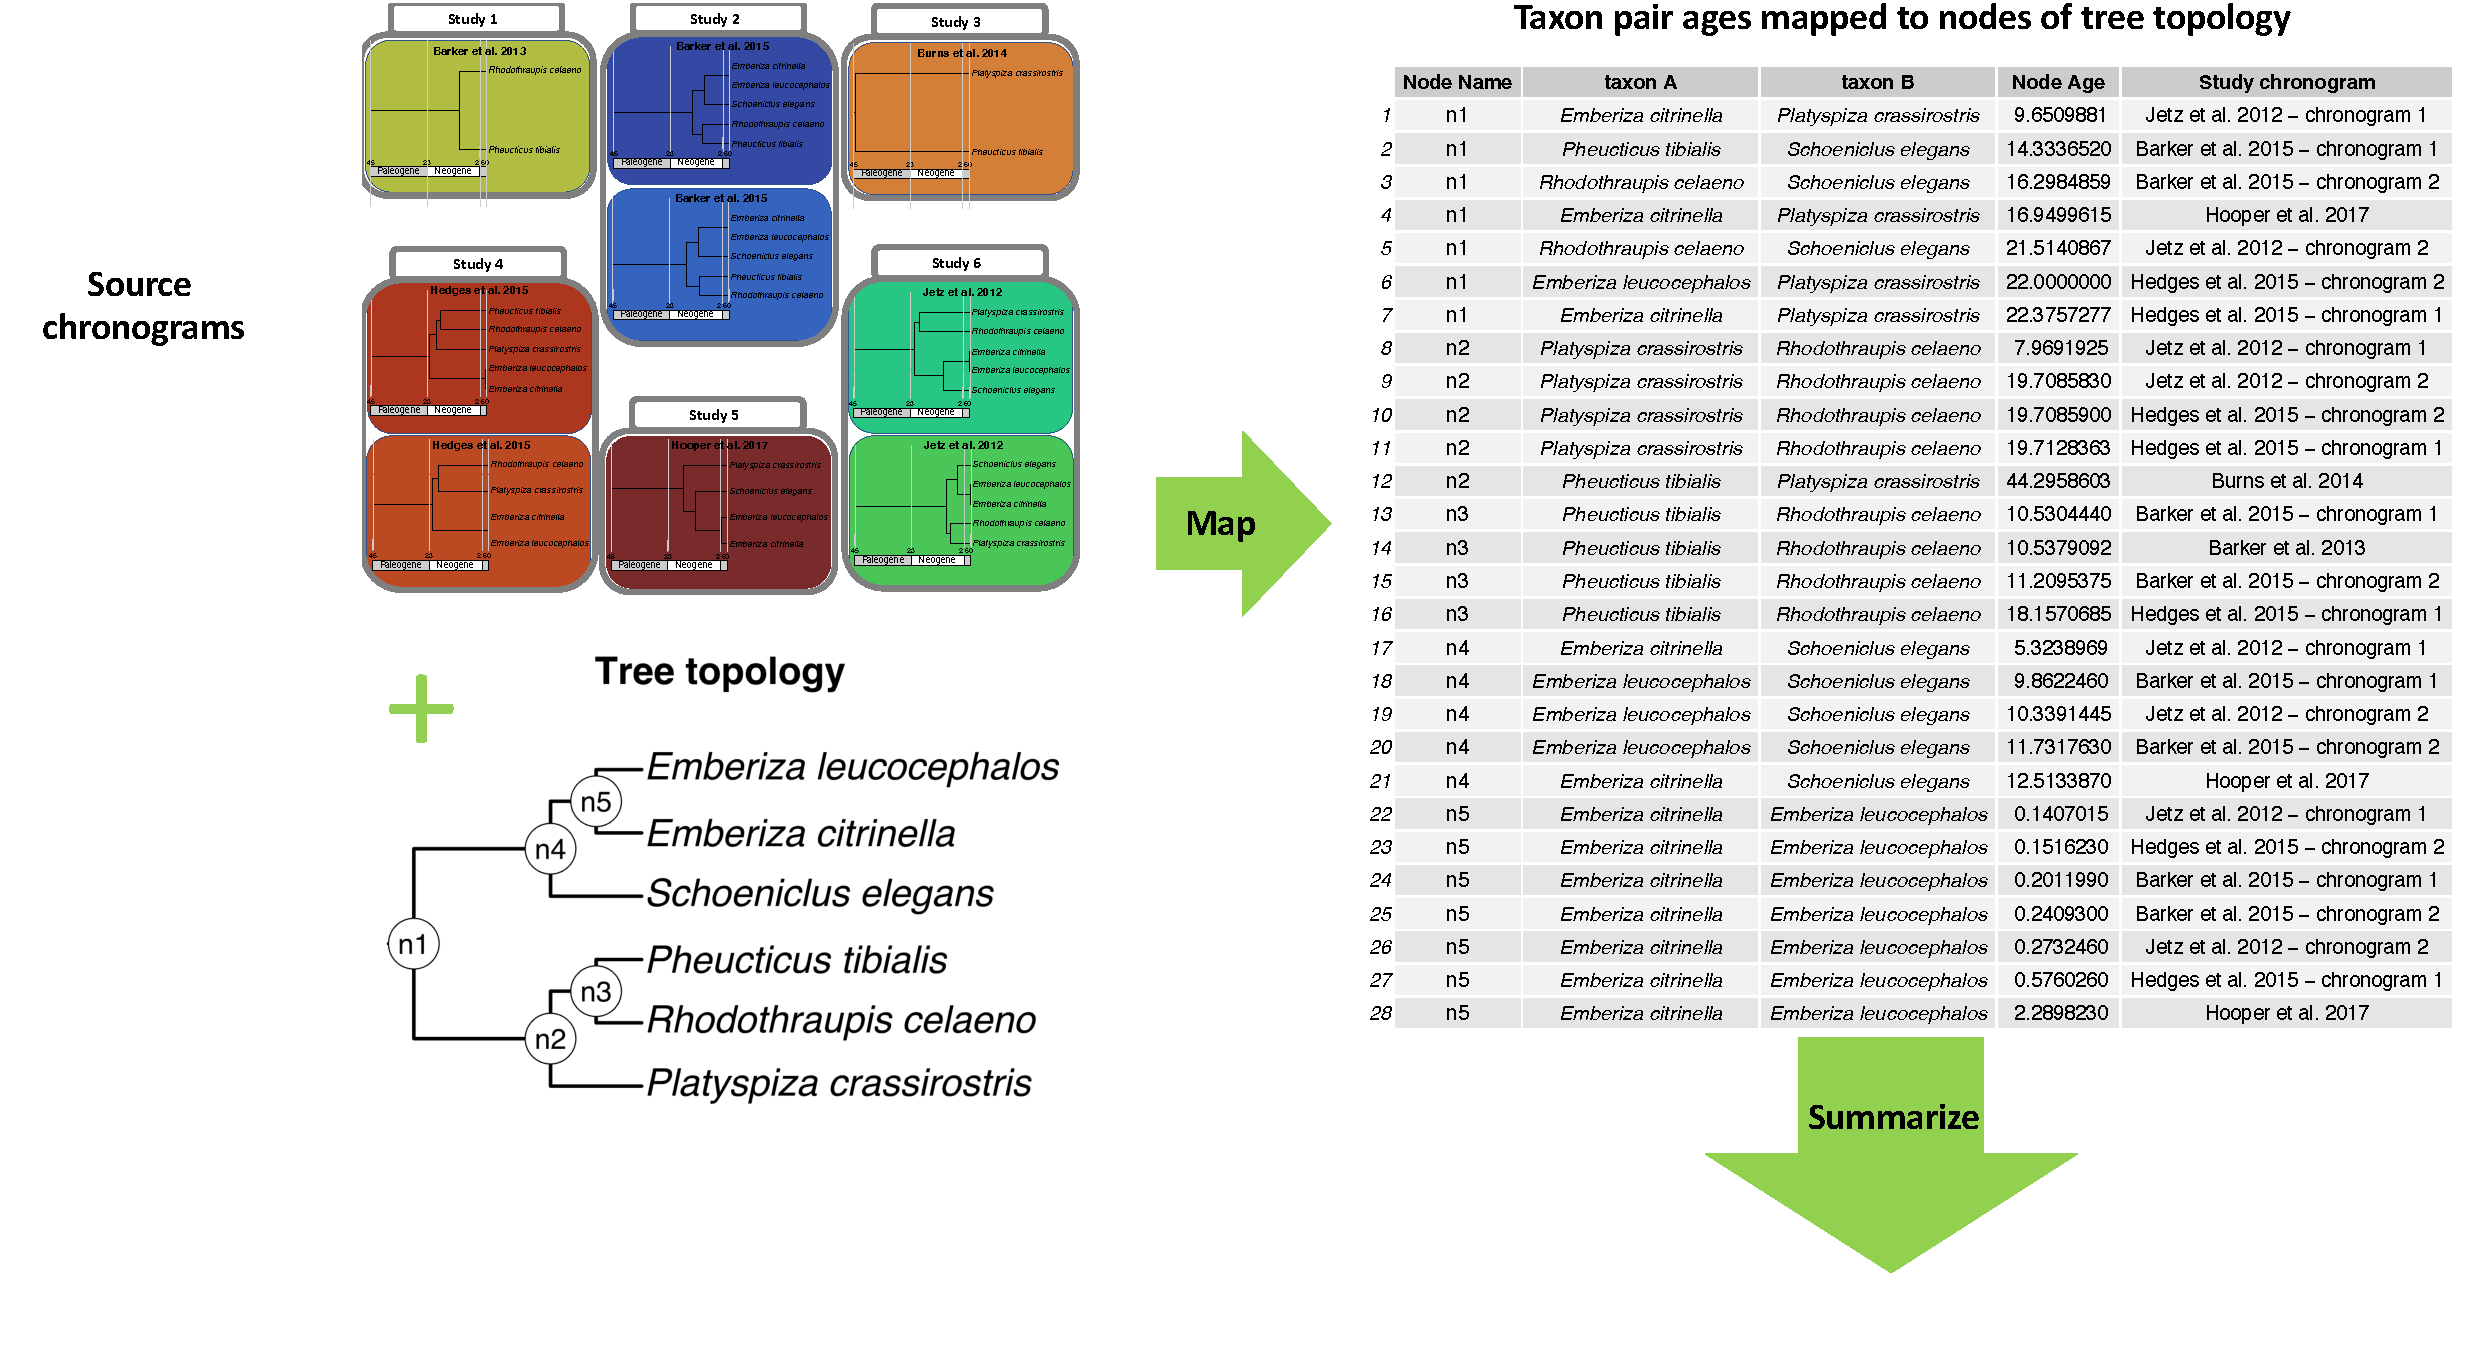
\includegraphics[width=1\linewidth]{../figures/figure2/figure2-1.pdf}
%\caption{Age data results of a DateLife search of a small sample of 6 %bird species within the Passeriformes. Input names were found across 9 %chronograms within 6 independent studies (Barker et al. %(\protect\hyperlink{ref-barker2012going}{2012}), Barker et al. %(\protect\hyperlink{ref-barker2015new}{2015}), Burns et al. %(\protect\hyperlink{ref-burns2014phylogenetics}{2014}), Hedges et al. %(\protect\hyperlink{ref-Hedges2015}{2015}), Hooper and Price %(\protect\hyperlink{ref-hooper2017chromosomal}{2017}), Jetz et al. %(\protect\hyperlink{ref-Jetz2012}{2012}).) This revealed 28 age data %points for the queried species names.}
%\label{fig:figure2-1}
%\end{figure}
%
%%%%%%%%%%%%%%%%%%%%%%%%%%%%%%%%%%%%%%%%%%%%%%%%%%%%%%%%%%%%%%%%%%%
%%%%%%%%%%%%%%%%%%%%%%%%%    FIGURE 2-2  %%%%%%%%%%%%%%%%%%%%%%%%%%
%%%%%%%%%%%%%%%%%%%%%%%%%%%%%%%%%%%%%%%%%%%%%%%%%%%%%%%%%%%%%%%%%%%
%\begin{figure}[!h]
%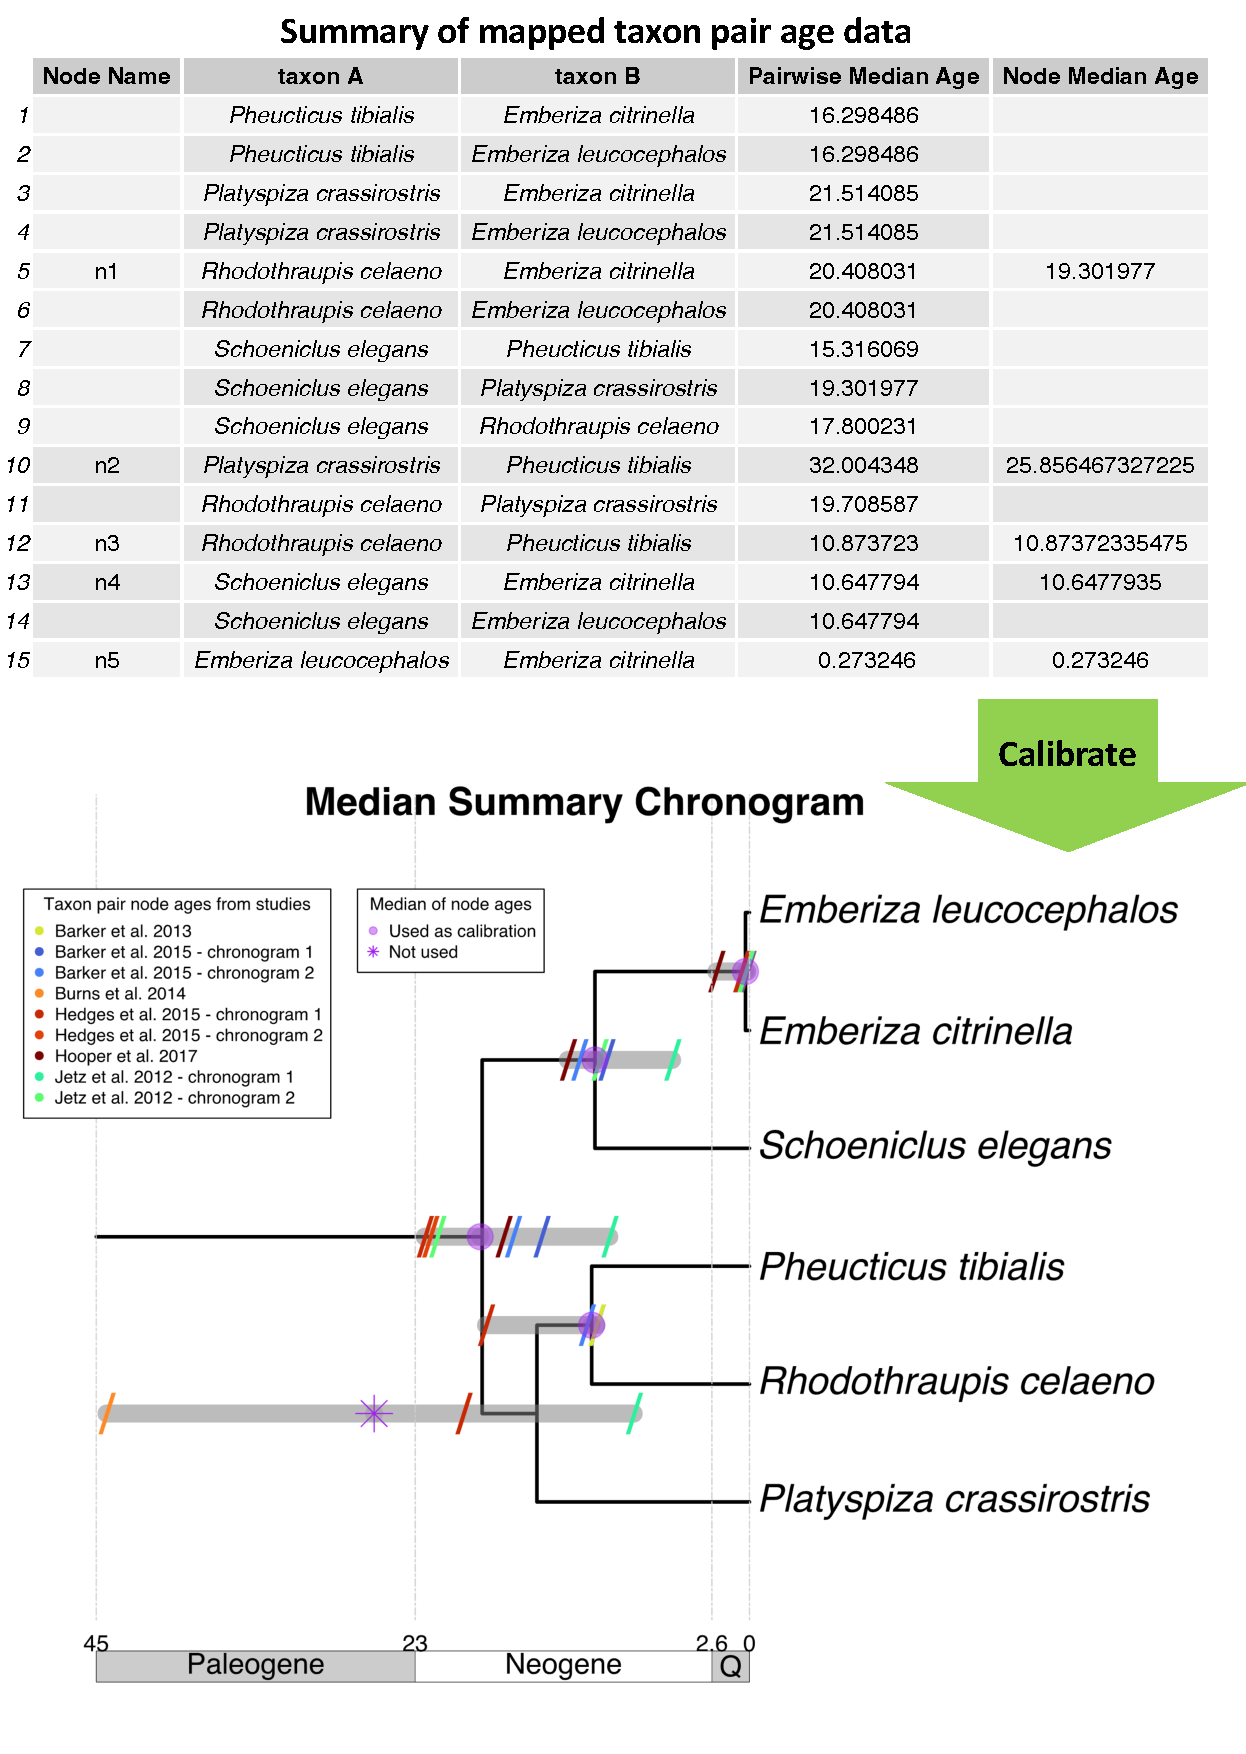
\includegraphics{../figures/figure2/figure2-2.pdf}
%\caption{Summarized age data is used as secondary calibrations to date %a tree topology as a summary chronogram.}
%\label{fig:summaries}
%\end{figure}


%%%%%%%%%%%%%%%%%%%%%%%%%%%%%%%%%%%%%%%%%%%%%%%%%%%%%%%%%%%%%%%%%%
%%%%%%%%%%%%%%%%%%%%%%%%    FIGURE 3    %%%%%%%%%%%%%%%%%%%%%%%%%%
%%%%%%%%%%%%%%%%%%%%%%%%%%%%%%%%%%%%%%%%%%%%%%%%%%%%%%%%%%%%%%%%%%
\begin{figure}[!h]
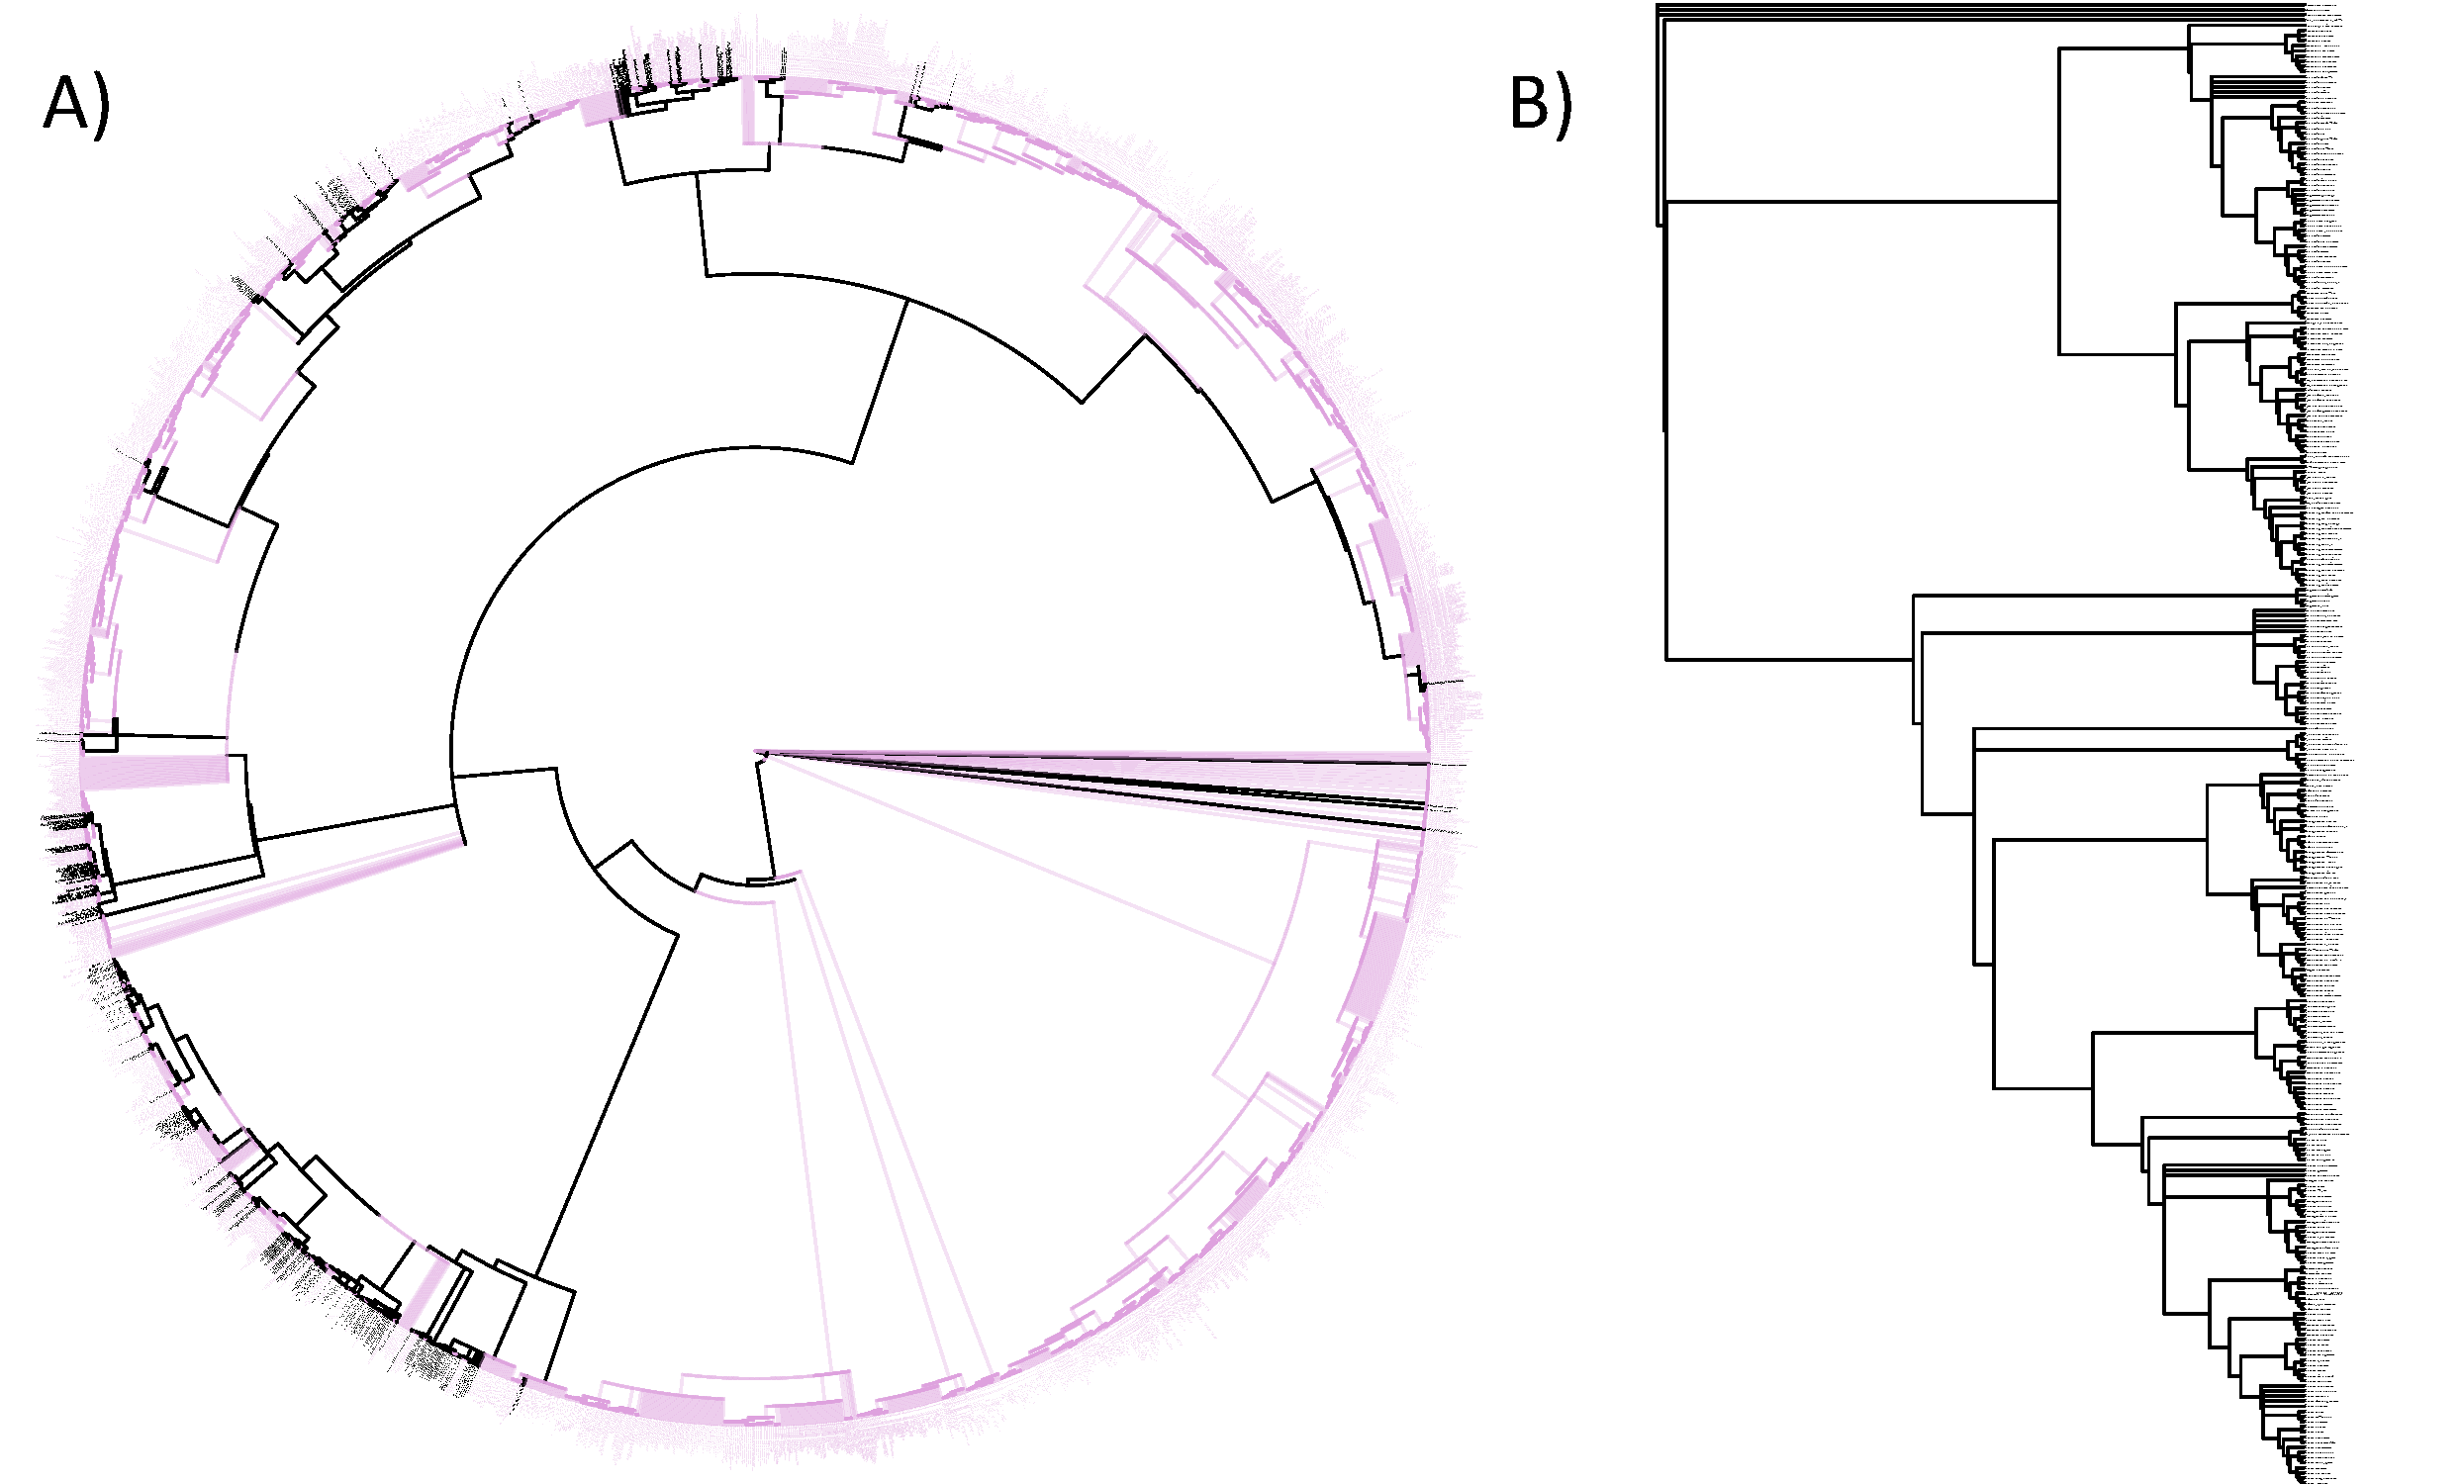
\includegraphics{../figures/fringillidae-topologies/fringillidae-topology.pdf}
\caption{Tree topologies obtained from Open Tree of Life's (OpenTree) synthetic phylogenetic tree. A) Topology of 2,333 tips and 1,305 internal nodes, encompassing bird species within the family Fringillidae following the NCBI taxonomy (black), as well as all other bird species that share the same mrca node in OpenTree's synthetic tree (purple). B) Topology of 289 tips and 253 internal nodes, encompassing bird species within the Fringillidae only, resulting from pruning purple branches from topology A.
Bird species within the Fringillidae do not form a monophyletic group
(Alström et al. \protect\hyperlink{ref-}{2014},
Barker, Cibois, Schikler, Feinstein, \& Cracraft \protect\hyperlink{ref-barker2004phylogeny}{2004},
Barker et al. \protect\hyperlink{ref-barker2013going}{2013},
Barker \protect\hyperlink{ref-barker2014mitogenomic}{2014},
Barker et al. \protect\hyperlink{ref-barker2015new}{2015},
Beresford, Barker, Ryan, \& Crowe \protect\hyperlink{ref-beresford2005african}{2005},
Bryson Jr et al. \protect\hyperlink{ref-bryson2014diversification}{2014},
Burleigh, Kimball, \& Braun \protect\hyperlink{ref-burleigh2015building}{2015},
Burns et al. \protect\hyperlink{ref-burns2014phylogenetics}{2014},
Chaves, Hidalgo, \& Klicka \protect\hyperlink{ref-chaves2013biogeography}{2013},
Claramunt \& Cracraft \protect\hyperlink{ref-claramunt2015new}{2015},
Gibb et al. \protect\hyperlink{ref-gibb2015new}{2015},
Hackett et al. \protect\hyperlink{ref-hackett2008phylogenomic}{2008},
Jetz et al. \protect\hyperlink{ref-Jetz2012}{2012},
Johansson, Fjeldså, \& Bowi \protect\hyperlink{ref-johansson2008phylogenetic}{200},
Kimball et al. \protect\hyperlink{ref-kimball2019phylogenomic}{2019},
Klicka et al. \protect\hyperlink{ref-klicka2014comprehensive}{2014},
Lamichhaney et al. \protect\hyperlink{ref-lamichhaney2015evolution}{2015},
Lerner, Meyer, James, Hofreiter, \& Fleischer \protect\hyperlink{ref-lerner2011multilocus}{2011},
Lovette et al. \protect\hyperlink{ref-lovette2010comprehensive}{2010},
Moyle et al. \protect\hyperlink{ref-moyle2016tectonic}{2016},
Ödeen, Håstad, \& Alström \protect\hyperlink{ref-odeen2011evolution}{2011},
Oliveros et al. \protect\hyperlink{ref-oliveros2019earth}{2019},
Päckert et al. \protect\hyperlink{ref-packert2012horizontal}{2012},
Parchman, Benkman, \& Mezquida \protect\hyperlink{ref-parchman2007coevolution}{2007},
Powell et al. \protect\hyperlink{ref-powell2014comprehensive}{2014},
Price et al. \protect\hyperlink{ref-price2014niche}{2014},
Pulgarín-R, Smith, Bryson Jr, Spellman, \& Klicka \protect\hyperlink{ref-pulgarin2013multilocus}{2013},
Selvatti, Gonzaga, \& Moraes Russo \protect\hyperlink{ref-selvatti2015paleogene}{2015},
Tietze, Päckert, Martens, Lehmann, \& Sun \protect\hyperlink{ref-tietze2013complete}{2013},
Treplin et al. \protect\hyperlink{ref-treplin2008molecular}{2008},
Zuccon, Prŷs-Jones, Rasmussen, \& Ericson \protect\hyperlink{ref-zuccon2012phylogenetic}{2012}).
}
\label{fig:fringillidae-topologies}
\end{figure}


%%%%%%%%%%%%%%%%%%%%%%%%%%%%%%%%%%%%%%%%%%%%%%%%%%%%%%%%%%%%%%%%%%
%%%%%%%%%%%%%%%%%%%%%%%%    FIGURE 4    %%%%%%%%%%%%%%%%%%%%%%%%%%
%%%%%%%%%%%%%%%%%%%%%%%%%%%%%%%%%%%%%%%%%%%%%%%%%%%%%%%%%%%%%%%%%%
\begin{figure}[!h]
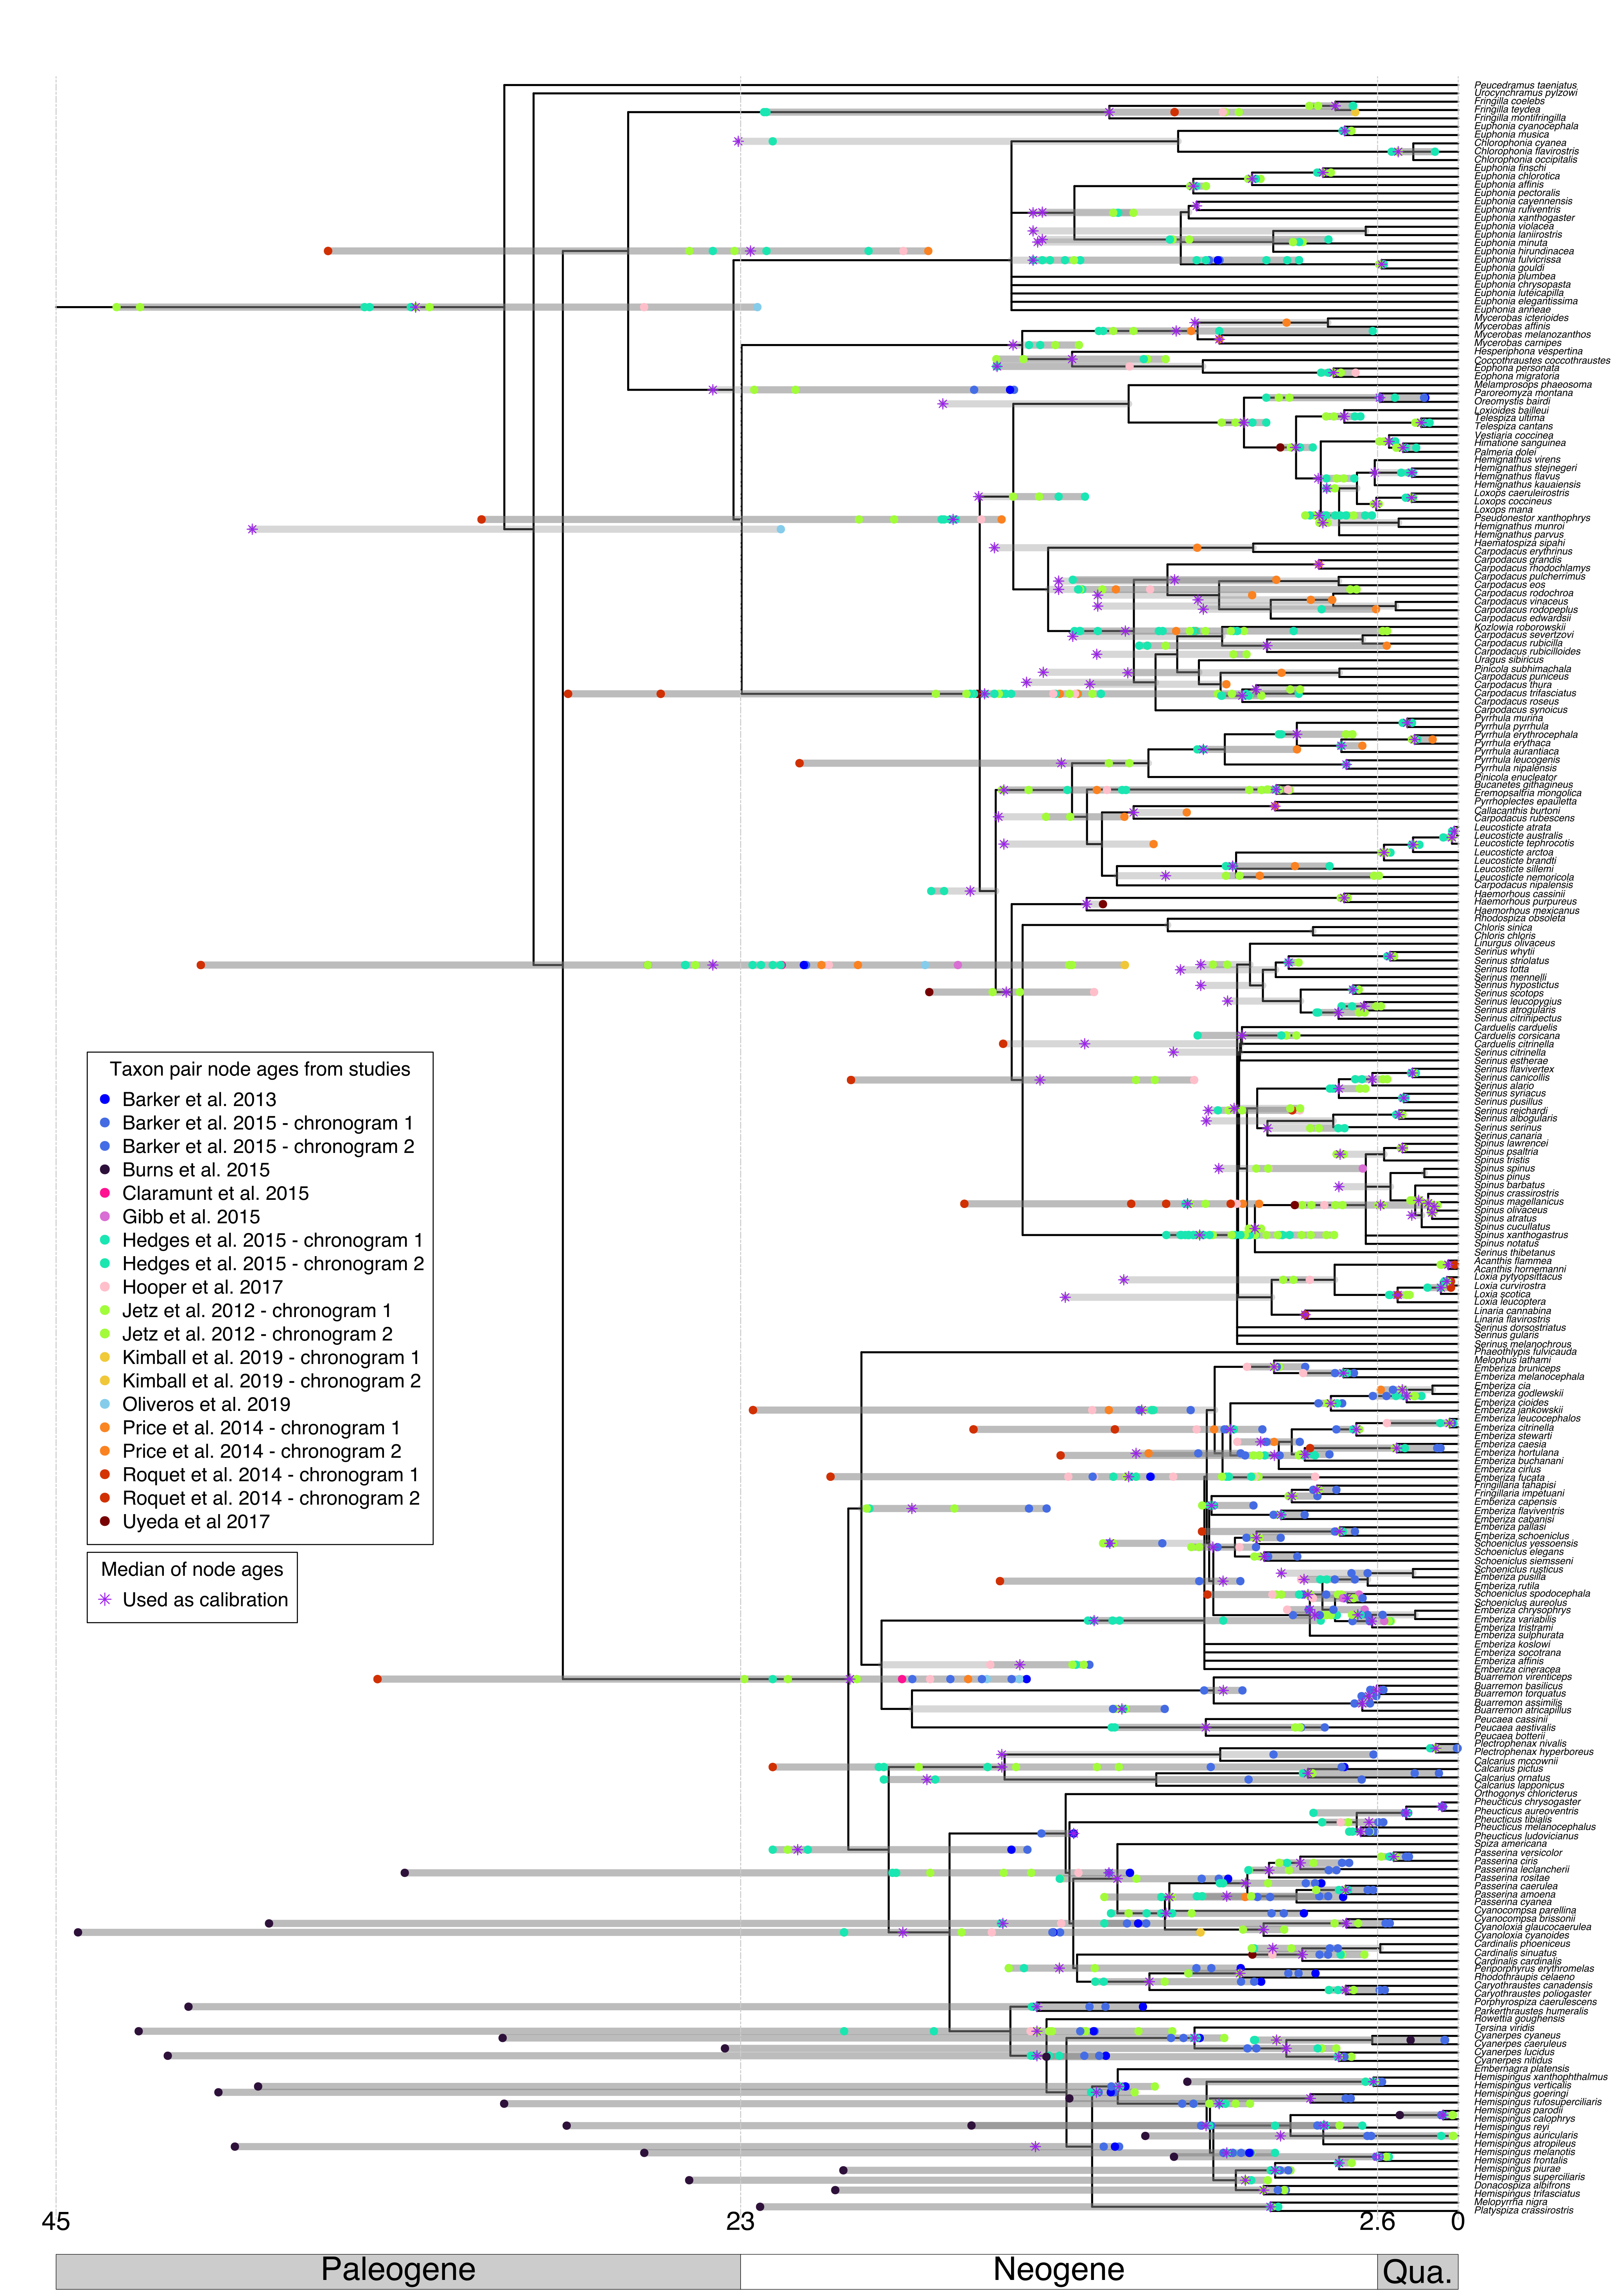
\includegraphics{../figures/figure-fringillidae/median_and_calibration_ages_simple.png}
\caption{Fringillidae median summary chronogram generated with DateLife. It has 256 tips and 233 nodes.}
\label{fig:fringillidages}
\end{figure}
